\documentclass{beamer}
%\usetheme{AnnArbor}
\usetheme{Madrid}
% \usecolortheme{default}
\usecolortheme{beaver} % Change color theme to red
% Title Page
\title[Tight Frames and Matroids]{Tight Frames and Matroids}
\author{Kai Chun Lin}
\institute{Rose-Hulman Institute of Technology}
\setbeamertemplate{footline}{%
  \leavevmode%
  \hbox{%
    \begin{beamercolorbox}[wd=.33\paperwidth,ht=2.25ex,dp=1ex,center]{author in head/foot}%
      \usebeamerfont{author in head/foot}\insertshortauthor\ (Rose-Hulman)
    \end{beamercolorbox}%
    \begin{beamercolorbox}[wd=.33\paperwidth,ht=2.25ex,dp=1ex,center]{title in head/foot}%
      \usebeamerfont{title in head/foot}\insertshorttitle
    \end{beamercolorbox}%
    \begin{beamercolorbox}[wd=.34\paperwidth,ht=2.25ex,dp=1ex,center]{date in head/foot}%
      \usebeamerfont{date in head/foot}\insertshortdate{}\hspace*{2em}
      \insertframenumber{} / \inserttotalframenumber\hspace*{2ex}
    \end{beamercolorbox}}%
  \vskip0pt%
}
\usepackage{amsmath,amssymb,amsthm}
\newcommand{\RR}{\mathbb{R}}

\usepackage{tikz, pgfplots}
\usetikzlibrary{arrows, calc}
\pgfplotsset{compat=1.18}

\usepackage{mathtools}
\DeclarePairedDelimiter\set{\{}{\}}
\usepackage{multicol}
\usepackage[backend=biber]{biblatex}
\addbibresource{library.bib}

\newtheorem{conjecture}{Conjecture}
\renewcommand{\vec}[1]{\mathbf{#1}}
\newcommand{\ivec}[2][.8]{%
  \scalebox{#1}{%
    \renewcommand{\arraystretch}{.8}%
    $\begin{bmatrix}#2\end{bmatrix}$%
  }
}
\usebackgroundtemplate{
\ifnum\thepage=1
    \begin{tikzpicture}[overlay, remember picture]
      \node[anchor=north east, inner sep=0pt] at ([xshift = -96pt,yshift=7pt]current page.north east) {\includegraphics[width=6cm]{Photo/Rose+Hulman+Logo.png}};
    \end{tikzpicture}
    \else
  \begin{tikzpicture}[overlay, remember picture]
    \node[anchor=north east, inner sep=17pt] at ([xshift=65pt]current page.north east) {\includegraphics[width=6cm]{Photo/Rose+Hulman+Logo.png}};
  \end{tikzpicture}
  \fi
}
\setbeamercolor{title page}{fg=black,bg=red}
\date{ April 6, 2024}

\begin{document}

\begin{frame}
  \titlepage
\end{frame}

% Outline
\begin{frame}{Outline}
  \tableofcontents
\end{frame}

% % Sample Slide
% \section{Introduction}
% \begin{frame}{Introduction}
%   \begin{itemize}
%     \item Brief overview of the topic
%     \item Objectives of the presentation
%   \end{itemize}
% \end{frame}

% Main Content
\section{Introduction of Matroid, Frame and Tight Frame}
\begin{frame}{Introduction of Matroid}
 \begin{itemize}
    \item <1- >Matroid is a generalization of linearly independent set
    % \item A finite matroid $M$ is a pair $(E, \mathcal{I})$, where E is a finite set\\
    % (referred to as the ground set) and $\mathcal{I}$ is a collection of subsets of $E$ (referred to as the independent sets), satisfying the three axioms.
    % \cite{datta2019low}
    \item <2- > A \textbf{matroid} is a pair $(S,I)$ with $S$ being a \textbf{ground set} and $I$ is a family of subsets of $S$  which is called (\textbf{Independent Subsets})such that it satisfy 3 axioms.
    \item <3- > Axioms
        \begin{enumerate}
            \item <4- > The empty set is independent $\emptyset \in \textit{I}$
        \item <5- > Every subset of an independent set is independent
        \item <6- > (Exchange Property) If $A$ and $B$ are two independent sets (i.e., each set is independent) and $A$ has more elements than $B$, then there exists $x \in A \setminus B$ such that $B \cup \{x\}$ is in $\mathcal{I}$.
        \cite{oxley2003matroid}

        \end{enumerate}
        
  \end{itemize}
\end{frame}

\begin{frame}{Introduction of  Graphic Matroid}
\begin{figure}
  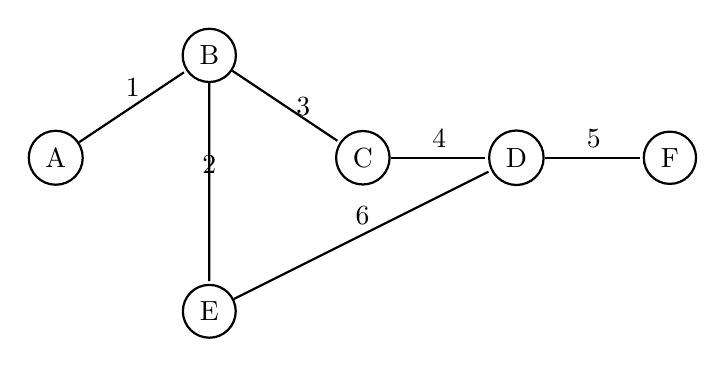
\begin{tikzpicture}[>=stealth',shorten >=1pt,auto,node distance=3cm,thick,scale=0.65]
  % Define nodes
  \node[circle, draw] (A) at (0,0) {A};
  \node[circle, draw] (B) at (3,2) {B};
  \node[circle, draw] (C) at (6,0) {C};
  \node[circle, draw] (D) at (9,0) {D};
  \node[circle, draw] (E) at (3,-3) {E};
  \node[circle, draw] (F) at (12,0) {F};
  
  % Draw edges with labels
  \draw (A) edge node[above] {1} (B);
  \draw (B) edge node[above] {2} (E);
  \draw (B) edge node[right] {3} (C);
  \draw (C) edge node[above] {4} (D);
  \draw (E) edge node[above] {6} (D);
  \draw (D) edge node[above] {5} (F);
\end{tikzpicture}
% \caption{Caption?}
\end{figure}
\begin{itemize}
    \item <1-> Simple graphs such as this define \textit{graphic matroids}.
    \item <2-> Dependent sets are sets of edges that contain circuits.
\end{itemize}
\end{frame}

{
\usebackgroundtemplate{}
\begin{frame}{Ground set, Independent sets, Dependent sets}
    
    \begin{itemize}
       \item <1- >In this graph the \textbf{groundset} $S =\{1,2,3,4,5,6\}$ and \textit{maximal} independent sets are
       \[
            M = \{\{1, 2, 3, 5, 6\}, \{1, 3, 4, 5, 6\}, ...\}
       \]
    %    \[I = \{ \begin{aligned}
    %     &\emptyset , \{1\} , \{2\} , \dots ,\{6\} ,
    % \{1,2\} , \{1,3\}, \dots \\
    %   &\{1,3,2,6,5\} , \{1,3,4,6,5\} ,\{1,2,6,4,5\} , \{1,2,3,4,5\}
    % \}
    % \end{aligned}\]
        % \item Independent sets are collections without cycles why?
        \item <2- > Example of Independent set $\{1,2,3,5\} , \{3,2,1\}$
        \item <3- > Example of Dependent set $\{2,3,4,6\}$
        
    \end{itemize}
    % Does anyone know what is the example of dependent set?

\end{frame}

\begin{frame}{Some Terminology of Matroid}
   \begin{figure}
  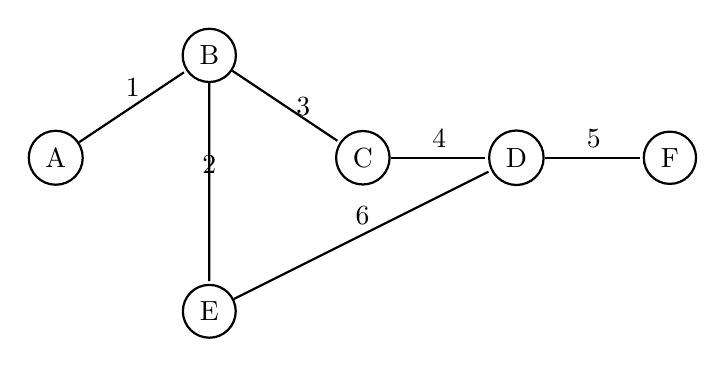
\begin{tikzpicture}[>=stealth',shorten >=1pt,auto,node distance=3cm,thick,scale=0.65]
  % Define nodes
  \node[circle, draw] (A) at (0,0) {A};
  \node[circle, draw] (B) at (3,2) {B};
  \node[circle, draw] (C) at (6,0) {C};
  \node[circle, draw] (D) at (9,0) {D};
  \node[circle, draw] (E) at (3,-3) {E};
  \node[circle, draw] (F) at (12,0) {F};
  
  % Draw edges with labels
  \draw (A) edge node[above] {1} (B);
  \draw (B) edge node[above] {2} (E);
  \draw (B) edge node[right] {3} (C);
  \draw (C) edge node[above] {4} (D);
  \draw (E) edge node[above] {6} (D);
  \draw (D) edge node[above] {5} (F);
\end{tikzpicture}
% \caption{Caption?}
\end{figure}
    \begin{itemize}

        \item <1- > A \textbf{maximal} independent set is called a \textbf{base}.
        \item <2- > Every \textbf{base} of a given matroid has the same size.
       
        %\item <3- > Can you think some examples of base for the previous graph?
        \item <3 -> $\{1,3,2,6,5\} , \{1,3,4,6,5\} , \{1,2,6,4,5\}$ these are bases of the graph.
        \item <4- > The \textbf{rank} of a matroid is the size of any base.
        \item <5- > A \textbf{circuit} is a minimal dependent set.
    \end{itemize}
\end{frame}
}

% \begin{frame}{Example of Matroid}
%     \[A = \begin{bmatrix}
%     1 & 0 & 0 & 1 & 1 & 0 \\
%     0 & 1 & 0 & 1 & 0 & 1 \\
%     0 & 0 & 1 & 0 & 1 & 1
%     \end{bmatrix}\]
%     \[E = \{1,2,3,4,5,6 \}\]

%     \begin{itemize}
%         \item <1-> Independent sets are
%         \[
%         \{\emptyset, \{1\}, \{2\}, \{3\}, \{1,2\}, \{1, 3\}, \{2, 3\}, \{1, 2, 3\}\}.
%         \]
%     \end{itemize}
% \end{frame}

\begin{frame}{Application of Matroid}

%     \item Matroids seem very mathematical, but they can model many real problems. Many graph
% theory problems can be restated in matroid language using the construction above, and the
% restatement of famous graph algorithms – Kruskal’s minimum weight spanning tree or finding
% a matching in a graph – have very natural interpretations. Similarly, we can (and do!) go
% the other way. Proving statements for matroids also proves them for all the objects matroids
% generalize, and this is a very powerful tool in mathematics
\begin{itemize}
    \item geometry
    \item topology
    \item combinatorial optimization
    \item network theory
    \item coding theory
    \\
    \cite{neel2009matroids}
    \cite{kashyap2009applications}
\end{itemize}
    
\end{frame}


\begin{frame}{Introduction of Frame}
  \begin{itemize}
    % \item Frames are collections of vectors that can approximate any vector in the space with arbitrary accuracy, allowing for redundancy in representation.
    
    \item In linear algebra, a frame of an inner product space is a generalization of a basis of a vector space to sets that may be linearly dependent.\cite{kovavcevic2008introduction}
    
    \item In finite-dimensional vector spaces, frames are spanning sets.
    %Frame_Motion_Signal_Processing
    \item In the signal processing, a frame provides a redundant, stable way of representing a signal.\cite{goyal2001quantized}
    
  \end{itemize}
\end{frame}

\begin{frame}{Example of Frame}
  \begin{itemize}
    \item <1-> Let
    \[
        \vec{f}_1 = \ivec{1\\1}, \vec{f}_2 = \ivec{1\\-1}, \vec{f}_3 = \ivec{0\\1}.
    \]
    This is a frame for $\RR^2$ since it's a spanning set (as $\operatorname{rank}(\ivec{\vec{f}_1 & \vec{f}_2 & \vec{f}_3}) = 2$).

    \item <2-> Any other vector $\vec{v}\in\RR^2$ can be written as a linear combination of the frame vectors:
    \[
        \vec{v} = c_1\vec{f}_1 + c_2\vec{f}_2 + c_3\vec{f}_3
    \]

    \item <3-> Since this frame is linearly dependent, this can be done in infinitely many ways.
  \end{itemize}
\end{frame}

\begin{frame}{Application of Frame}
  \begin{itemize}
    % \item Frames are used in error detection and correction and the design and analysis of filter banks and more generally in applied mathematics, computer science, and engineering.

  \item Signal Processing
  % : Frames are used for signal denoising, compression, and reconstruction. They provide a flexible framework for representing signals in various domains, such as time, frequency, or spatial.
  
  \item Image Processing
  % : Frames are employed for image compression, enhancement, and restoration. They enable efficient representation of image patches and facilitate robust image reconstruction from incomplete or noisy data.
  
  \item Data Compression
  % : Frames play a crucial role in data compression techniques, such as JPEG and MP3. By exploiting the redundancy inherent in signals or images, frames allow for efficient encoding and decoding processes.
  
  \item Sensing and Sampling
  % : Frames are utilized in sensor networks and sampling schemes for signal acquisition and reconstruction. They enable the design of sampling matrices that satisfy specific sensing or recovery properties.
  
  \item Communications
  % : Frames are used in communication systems for channel coding, modulation, and equalization. They enable reliable transmission of information over noisy or bandwidth-limited channels.
  
  \cite{casazza2012finite}
  \end{itemize}
\end{frame}



\begin{frame}
    \frametitle{Bases and erasures}
    \begin{multicols}{2}
        \begin{itemize}
            \item <1-> Let $\set{\vec{e}_{i}}_{i=1}^{2}$ denote the (orthonormal) basis given by $\vec{e}_{1} = \ivec{1\\0},\vec{e}_{2} = \ivec{0\\1}$.
            Let $\vec{x} = 2\vec{e}_{1}+3\vec{e}_{2}$.
            
            \item <2-> If sender transmits $2,3$ successfully to receiver, then $\vec{x}$ can be reconstructed.

            \item <3-> Suppose only $2$ is successfully transmitted. 
            Receiver then constructs the vector $\hat{\vec{x}} = \ivec{2\\0}$.

        \end{itemize}
        \columnbreak
        \only<1>{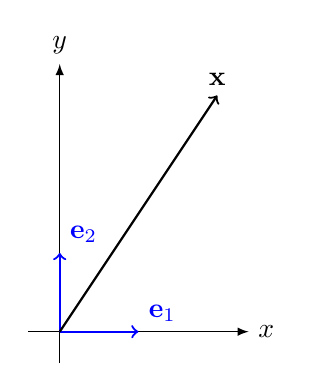
\begin{tikzpicture}
            \coordinate (O)   at (0,0);
            \coordinate (XAxisMin) at (-.4,0);
            \coordinate (XAxisMax) at (2.4,0);
            \coordinate (YAxisMin) at (0,-.4);
            \coordinate (YAxisMax) at (0,3.4);
            \draw [thin, black,-latex] (XAxisMin) -- (XAxisMax) node[right] {$x$};% Draw x axis
            \draw [thin, black,-latex] (YAxisMin) -- (YAxisMax) node[above] {$y$};% Draw y axis
    
            \draw[blue, thick, ->] (O)--(1,0) node[above right] {$\vec{e}_{1}$};
            \draw[blue, thick, ->] (O)--(0,1) node[above right] {$\vec{e}_{2}$};
    
            % \draw[blue, thick, ->] (O)--(1,0) node[above right] {$\vec{e}_{1}$};
            % \draw[blue, thick, ->] (O)--(0,1) node[above right] {$\vec{e}_{2}$};

            % \node at (2,3) {$\bullet$};
            \draw[black, thick, ->] (O)--(2,3) node[above] {$\vec{x}$};
        \end{tikzpicture}}
        \only<2>{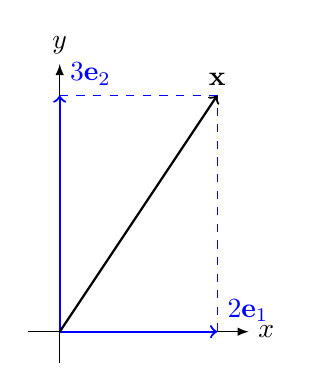
\begin{tikzpicture}
            \coordinate (O)   at (0,0);
            \coordinate (XAxisMin) at (-.4,0);
            \coordinate (XAxisMax) at (2.4,0);
            \coordinate (YAxisMin) at (0,-.4);
            \coordinate (YAxisMax) at (0,3.4);
            \draw [thin, black,-latex] (XAxisMin) -- (XAxisMax) node[right] {$x$};% Draw x axis
            \draw [thin, black,-latex] (YAxisMin) -- (YAxisMax) node[above] {$y$};% Draw y axis
    
            % \draw[blue, ultra thick, ->] (O)--(1,0) node[above right] {$\vec{e}_{1}$};
            % \draw[blue, ultra thick, ->] (O)--(0,1) node[above right] {$\vec{e}_{2}$};
    
            \draw[blue, thick, ->] (O)--(2,0) node[above right] {$2\vec{e}_{1}$};
            \draw[blue, thick, ->] (O)--(0,3) node[above right] {$3\vec{e}_{2}$};
            \draw[blue, dashed] (2,0)--(2,3);
            \draw[blue, dashed] (0,3)--(2,3);
            % \node at (2,3) {$\bullet$};
            \draw[black, thick, ->] (O)--(2,3) node[above] {$\vec{x}$};
        \end{tikzpicture}}
        \only<3->{\begin{tikzpicture}
            \coordinate (O)   at (0,0);
            \coordinate (XAxisMin) at (-.4,0);
            \coordinate (XAxisMax) at (2.4,0);
            \coordinate (YAxisMin) at (0,-.4);
            \coordinate (YAxisMax) at (0,3.4);
            \draw [thin, black,-latex] (XAxisMin) -- (XAxisMax) node[right] {$x$};% Draw x axis
            \draw [thin, black,-latex] (YAxisMin) -- (YAxisMax) node[above] {$y$};% Draw y axis
    
            % \draw[blue, ultra thick, ->] (O)--(1,0) node[above right] {$\vec{e}_{1}$};
            % \draw[blue, ultra thick, ->] (O)--(0,1) node[above right] {$\vec{e}_{2}$};
    
            % \draw[blue, thick, ->] (O)--(2,0) node[above right] {$2\vec{e}_{1}$};
            % \draw[blue, thick, ->] (O)--(0,3) node[above right] {$3\vec{e}_{2}$};
            % \draw[blue, dashed] (2,0)--(2,3);
            % \draw[blue, dashed] (0,3)--(2,3);
            % \node at (2,0) {$\bullet$};
            \draw[black, thick, ->] (O)--(2,3) node[above] {$\vec{x}$};
            \draw[red, thick, ->] (O)--(2,0) node[above] {$\hat{\vec{x}}$};
        \end{tikzpicture}}
    \end{multicols}
    \begin{itemize}
        \item <4-> Impossible to accurately reconstruct $\vec{x}$ if a (nonzero) coefficient is lost!
        Problem is that a basis has no redundancy.
    \end{itemize}
\end{frame}

\begin{frame}
    \frametitle{Frames and erasures}
    \begin{multicols}{2}
        \begin{itemize}
            \item <1-> Let 
            \[
                \vec{f}_{1} = \ivec{0\\1},\vec{f}_{2} = \ivec{-\frac{\sqrt{3}}{2} \\ -\frac{1}{2}}, \vec{f}_{3} = \ivec{\frac{\sqrt{3}}{2} \\ -\frac{1}{2}}.
            \]
            $\set{\vec{f}_{i}}_{i=1}^{3}$ is a frame for $\RR^{2}$.
            
            \item <2-> Let $\vec{x} = \ivec{2\\3}$.
            Then $\vec{x} = 2\vec{f}_{1} - (\frac{2}{\sqrt{3}} + 1)\vec{f}_{2} + (\frac{2}{\sqrt{3}} - 1)\vec{f}_{3}$.

            \item <3-> Suppose only $2$ and $-(\frac{2}{\sqrt{3}}+1)$ are successfully transmitted. 
            Receiver then constructs the vector $\hat{\vec{x}} = 2\vec{f}_{1} - (\frac{2}{\sqrt{3}} + 1)\vec{f}_{2}$.

        \end{itemize}
        \columnbreak
        \only<1>{\begin{tikzpicture}
            \coordinate (O)   at (0,0);
            \coordinate (XAxisMin) at (-1.4,0);
            \coordinate (XAxisMax) at (2.4,0);
            \coordinate (YAxisMin) at (0,-.4);
            \coordinate (YAxisMax) at (0,3.4);

            \draw [thin, black,-latex] (XAxisMin) -- (XAxisMax) node[right] {$x$};% Draw x axis
            \draw [thin, black,-latex] (YAxisMin) -- (YAxisMax) node[above] {$y$};% Draw y axis
            \draw[blue, thick, ->] (O)--(0,1) node[above right] {$\vec{f}_{1}$};
            \draw[blue, thick, ->] (O)--(-{sqrt(3)/2},-1/2) node[left] {$\vec{f}_{2}$};
            \draw[blue, thick, ->] (O)--({sqrt(3)/2},-1/2) node[right] {$\vec{f}_{3}$};
        \end{tikzpicture}}
        \only<2>{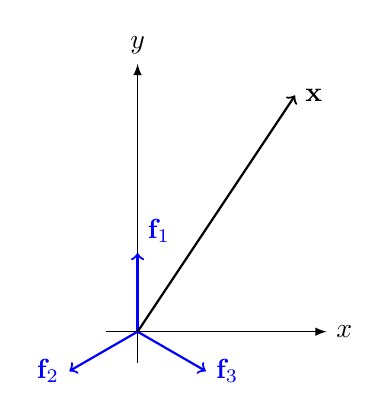
\begin{tikzpicture}
            \coordinate (O)   at (0,0);
            \coordinate (XAxisMin) at (-.4,0);
            \coordinate (XAxisMax) at (2.4,0);
            \coordinate (YAxisMin) at (0,-.4);
            \coordinate (YAxisMax) at (0,3.4);
            \draw [thin, black,-latex] (XAxisMin) -- (XAxisMax) node[right] {$x$};% Draw x axis
            \draw [thin, black,-latex] (YAxisMin) -- (YAxisMax) node[above] {$y$};% Draw y axis
    
            \draw[blue, thick, ->] (O)--(0,1) node[above right] {$\vec{f}_{1}$};
            \draw[blue, thick, ->] (O)--(-{sqrt(3)/2},-1/2) node[left] {$\vec{f}_{2}$};
            \draw[blue, thick, ->] (O)--({sqrt(3)/2},-1/2) node[right] {$\vec{f}_{3}$};
            \draw[black, thick, ->] (O)--(2,3) node[right] {$\vec{x}$};
        \end{tikzpicture}}
        \only<3->{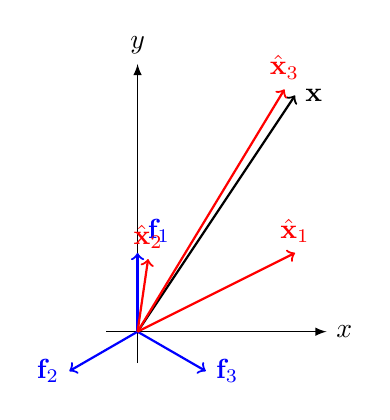
\begin{tikzpicture}
            \coordinate (O)   at (0,0);
            \coordinate (XAxisMin) at (-.4,0);
            \coordinate (XAxisMax) at (2.4,0);
            \coordinate (YAxisMin) at (0,-.4);
            \coordinate (YAxisMax) at (0,3.4);

            \coordinate (f1) at (0,1);
            \coordinate (f2) at (-{sqrt(3)/2},-1/2);
            \coordinate (f3) at ({sqrt(3)/2},-1/2);
            \coordinate (Xhat3) at ($2*(f1)-{2/sqrt(3)}*(f2)-(f2)$);
            \coordinate (Xhat1) at ($-{2/sqrt(3)}*(f2)-(f2) + {2/sqrt(3)}*(f3)-(f3)$);
            \coordinate (Xhat2) at ($(f1) + {2/sqrt(3)}*(f3)-(f3)$);
            % \coordinate (Yhat) at ($2*(f1)+{2/sqrt(3)}*(f3)-(f3)$);
            % \coordinate (Zhat) at ($-{2/sqrt(3)}*(f2)-(f2)+{2/sqrt(3)}*(f3)-(f3)$);
            \draw [thin, black,-latex] (XAxisMin) -- (XAxisMax) node[right] {$x$};% Draw x axis
            \draw [thin, black,-latex] (YAxisMin) -- (YAxisMax) node[above] {$y$};% Draw y axis
    
            % \draw[blue, ultra thick, ->] (O)--(1,0) node[above right] {$\vec{e}_{1}$};
            % \draw[blue, ultra thick, ->] (O)--(0,1) node[above right] {$\vec{e}_{2}$};
    
            % \draw[blue, thick, ->] (O)--(2,0) node[above right] {$2\vec{e}_{1}$};
            % \draw[blue, thick, ->] (O)--(0,3) node[above right] {$3\vec{e}_{2}$};
            % \draw[blue, dashed] (2,0)--(2,3);
            % \draw[blue, dashed] (0,3)--(2,3);
            % \node at (2,0) {$\bullet$};
            \draw[blue, thick, ->] (O)--(0,1) node[above right] {$\vec{f}_{1}$};
            \draw[blue, thick, ->] (O)--(-{sqrt(3)/2},-1/2) node[left] {$\vec{f}_{2}$};
            \draw[blue, thick, ->] (O)--({sqrt(3)/2},-1/2) node[right] {$\vec{f}_{3}$};
            \draw[black, thick, ->] (O)--(2,3) node[right] {$\vec{x}$};
            \draw[red, thick, ->] (O)--(Xhat3) node[above] {$\hat{\vec{x}}_3$};
            \draw[red, thick, ->] (O)--(Xhat1) node[above] {$\hat{\vec{x}}_1$};
            \draw[red, thick, ->] (O)--(Xhat2) node[above] {$\hat{\vec{x}}_2$};
            % \draw[red, thick, ->] (O)--(Yhat) node[above] {$\hat{\vec{y}}$};
            % \draw[red, thick, ->] (O)--(Zhat) node[above] {$\hat{\vec{z}}$};
        \end{tikzpicture}}

    \end{multicols}
\end{frame}
{
\usebackgroundtemplate{}
\begin{frame}{Introduction to Tight Frames}
  \begin{itemize}
    \item <1-> Given a frame $F = \ivec{\vec{f}_1 & \ldots & \vec{f}_N}$ for $\RR^d$ and some arbitrary $\vec{v}\in\RR^d$, we want an easy way to find coefficients $c_i$ such that
    \[
        \vec{v} = \sum_{i=1}^{N}c_i\vec{f}_i.
    \]
    \item <2-> This can be done quickly if the frame is \textbf{tight}: $FF^{T} = \alpha I$.
    Then
    \begin{align*}
        \alpha\vec{v}
        &= FF^{T}\vec{v} \\
        &= \ivec{\vec{f}_1 & \ldots & \vec{f}_N}\ivec{\vec{f}_1^T \\ \vdots \\ \vec{f}_N^T}\vec{v} \\
        &= \sum_{i=1}^{N}\vec{f}_i\langle\vec{f}_i,\vec{v}\rangle
    \end{align*}
    \item <3-> For tight frames, $c_i = \frac{\langle\vec{f}_i,\vec{v}\rangle}{\alpha}$.
    If the frame is also unit-normed, then $\alpha = \frac{N}{d}$.
  \end{itemize}
\end{frame}
}
\begin{frame}{Example of a Tight Frame}
  \begin{itemize}
    \item <1-> Let 
    \[
        \vec{f}_{1} = \ivec{0\\1},\vec{f}_{2} = \ivec{-\frac{\sqrt{3}}{2} \\ -\frac{1}{2}}, \vec{f}_{3} = \ivec{\frac{\sqrt{3}}{2} \\ -\frac{1}{2}}.
    \]

    \item <2-> This is a tight frame for $\RR^2$ since $FF^{T} = \frac{3}{2}I$.

    \item <3-> Relatively easy way to compute coefficients in frame expansion:
    \[
        \ivec{1 \\ 1} = \frac{2}{3}\left(1\vec{f}_1 -\frac{\sqrt{3}+1}{2}\vec{f}_2 + \frac{\sqrt{3}-1}{2}\vec{f}_3\right).
    \]
  \end{itemize}
\end{frame}

\begin{frame}{Equiangular Tight Frames}
  \begin{itemize}
    \item <1-> An $(N,d)$ \textbf{equiangular tight frame} (ETF) is a unit-normed tight frame of $N$ vectors  in $d$ dimensions with the extra condition $|\langle\vec{f}_i,\vec{f}_j\rangle| = \mu$.
    \item <2-> Such frames have important properties in coding theory and signal processing.\cite{SH1}
    \item <3-> A $(d+1,d)$ ETF always exists (see last slide for an example).
    \cite{datta2016construction}
  \end{itemize}
\end{frame}


 {
\usebackgroundtemplate{}
%Research Result
\section{Result}
\begin{frame}
   \begin{theorem}[K. Lin, J. Oldroyd 2023]
%A $(d+1, d)$ ETF can be constructed by first constructing a corresponding Gram matrix $G$ using the formula
%Then we need to add together columns of this matrix taken k at a time to form the particular matroid.
Let $\{\vec{f}_i\}_{i=1}^{d+1}$ be a $(d+1,d)$ ETF with $\langle\vec{f}_i,\vec{f}_j\rangle = -\frac{1}{d}, i\neq j$.
This has only one circuit, namely, the set $\{1, 2, \ldots, d, d+1\}$.
% We found that if $k=d$ this matroid has only one circuit.
\end{theorem}
\begin{proof}
% Since in the case $k=d$. In the first, we will have $k+1$ vector and to pick $d$ vectors and add them together to get a new vector and add this new vector in the matroid.
Since $\langle\vec{f}_i,\vec{f}_j\rangle = -\frac{1}{d}, i\neq j$, it follows that $\sum_{i=1}^{d+1}\vec{f}_i = \vec{0}$.
Hence, $\{1,\ldots, d+1\}$ is a dependent set in the matroid associated with
\[
    F = \ivec{\vec{f}_1 & \ldots & \vec{f}_{d+1}}.
\]
As the vectors span $\RR^d$ and any single vector $\vec{f}_i$ can be written as a linear combination of the other $d$ vectors, we can also say that no subset of $\{\vec{f}_i\}$ of size $d$ is linearly independent.
In other words, every columns is a dependent set but if we remove any columns it will be independent set.
\end{proof}
\end{frame}

\begin{frame}
    \frametitle{Multi-angle tight frames}
    \begin{itemize}
    \item <1-> Let $\{\vec{f}_i\}_{i=1}^{d+1}$ be a $(d+1,d)$ ETF with $\langle\vec{f}_i,\vec{f}_j\rangle = -\frac{1}{d}, i\neq j$.
    
    \item <2-> Let $1\leq k\leq d$ and let $\Lambda = \{i_1, i_2, \ldots, i_k\}$ denote a subset of $\{1,\ldots, d+1\}$ of size $k$.
    We can use $\Lambda$ to define a new vector $\vec{g}$ in terms of the original frame vectors as follows:
    \[
    \vec{g} = \vec{f}_{i_1} + \cdots + \vec{f}_{i_{k}}.
    \]

    \item <3-> The set of all $N = \binom{d+1}{k}$ such vectors $\{\vec{g}_n\}_{n=1}^{N}$ forms a multi-angle frame.\cite{datta2019low}
    \end{itemize}
\end{frame}

\begin{frame}
    \frametitle{Multi-angle frame example}
    \begin{example}
        Let $\{\vec{f}_1, \vec{f}_2, \vec{f}_3\}$ denote the Mercedes-Benz frame.
        Let
        \[
        \{\Lambda_n\}_{n=1}^{3} = \{\Lambda_1, \Lambda_2, \Lambda_3\} = \{\{1, 2\}, \{1, 3\}, \{2, 3\}\}
        \]
        denote the collection of subsets of $\{1,2,3\}$ of size $k = 2$.
        Then the frame determined by $\{\Lambda_n\}$ is given by
        \[
        \vec{g}_1 = \vec{f}_1+\vec{f}_2 = -\vec{f}_3,\quad \vec{g}_2 = \vec{f}_1+\vec{f}_3 = -\vec{f}_2,\quad \vec{g}_3 = \vec{f}_2+\vec{f}_3 = -\vec{f}_1.
        \]
    \end{example}
    \begin{itemize}
    \item <2-> In matrix form, the above computation looks like
    \[
    \ivec{\vec{g}_1 & \vec{g}_2 & \vec{g}_3}
    = \ivec{\vec{f}_1 & \vec{f}_2 & \vec{f}_3}\ivec{1 & 1 & 0 \\ 1 & 0 & 1 \\ 0 & 1 & 1} = FK.
    \]
    \item <3-> Circuit $\{\vec{g}_1,\vec{g}_2,\vec{g}_3\}$ corresponds to $K$.
    \end{itemize}
\end{frame}

\begin{frame}
    \frametitle{Multi-angle frame example}
    \begin{example}
        Let
        \[
            \vec{f}_1 = \ivec{0\\0\\1}, \vec{f}_2 = \ivec{0\\-\frac{2\sqrt{2}}{3} \\ -\frac{1}{3}}, \vec{f}_3 = \ivec{-\sqrt{\frac{2}{3}} \\ \frac{\sqrt{2}}{3} \\ -\frac{1}{3}}, \vec{f}_4 = \ivec{\sqrt{\frac{2}{3}} \\ \frac{\sqrt{2}}{3} \\ -\frac{1}{3}}
        \]
        which is a $(4,3)$ ETF satisfying $\langle\vec{f}_i,\vec{f}_j\rangle = -\frac{1}{3}$ and $\vec{f}_1 + \cdots + \vec{f}_4 = \vec{0}$.
        Let
        \[
        \{\Lambda_n\}_{n=1}^{6} = \{\Lambda_1, \Lambda_2, \ldots, \Lambda_6\} = \{\{1, 2\}, \{1, 3\}, \ldots, \{3, 4\}\}
        \]
        % denote the collection of subsets of $\{1,2,3,4\}$ of size $k = 2$.
        Then the frame determined by $\{\Lambda_n\}$ is given by
        \[
        \vec{g}_1 = \vec{f}_1+\vec{f}_2,\quad \vec{g}_2 = \vec{f}_1+\vec{f}_3, \quad \ldots, \quad \vec{g}_6 = \vec{f}_3+\vec{f}_4.
        \]
    \end{example}
\end{frame}

\begin{frame}
    \frametitle{Multi-angle frame example}
    \begin{itemize}
    \item <1-> In matrix form, the above computation looks like
    \[
    \ivec{\vec{g}_1 & \ldots & \vec{g}_6}
    = \ivec{\vec{f}_1 & \vec{f}_2 & \vec{f}_3 & \vec{f}_4}\ivec{1 & 1 & 0 & 0 & 0 & 0\\ 1 & 0 & 0 & 1 & 1 & 0 \\ 0 & 1 & 0 & 1 & 0 & 1 \\ 0 & 0 & 1 & 0 & 1 & 1} = FK.
    \]
    \item <2-> Circuit $\{\vec{g}_1, \vec{g}_6\}$ corresponds to \textit{submatrix} $\widehat{K} = \ivec{1 & 0 \\ 1 & 0 \\ 0 & 1 \\ 0 & 1}$.
    \end{itemize}
\end{frame}

\begin{frame}
    \frametitle{Circuits of $k$-angle frame}
    \begin{theorem}
        Let $\{\vec{f}_i\}$ be $(d+1,d)$ ETF with pairwise inner products $-\frac{1}{d}$.
        Given $\{\Lambda_n\}_{n=1}^{N}$ where $1\leq k\leq d+1$, $N = \binom{d+1}{k}$, define
        \[
            \vec{g}_n = \sum_{m\in\Lambda_n}\vec{f}_m
        \]
        where $\{\Lambda_n\}$ denotes the collection of $\binom{d+1}{k}$ subsets of $\{1,\ldots, d+1\}$ of size $k$.
        Then the submatrices of $K$ that correspond to circuits of the matroid associated with $\{\vec{g}_n\}$ have a $1$ in each row.
    \end{theorem}
    \begin{itemize}
        \item This converse does no hold.
    \end{itemize}
\end{frame}
\begin{frame}
    \frametitle{Circuits of $k$-angle frame}
    \begin{proof}
        \begin{itemize}
            \item <1-> Circuits are minimal dependent subsets of $\{\vec{g}_n\}$.

            \item <2-> Dependent sets correspond to solutions of $FK\vec{x} = \vec{0}$ with $\vec{x}\neq\vec{0}$.
            Minimal dependent sets correspond to nonzero $\vec{x}$ with \textit{fewest} possible nonzero entries.

            \item <3-> Two cases: $K\vec{x}\neq\vec{0}$ or $K\vec{x} = \vec{0}$.
            First case forces $K\vec{x} = c\vec{1}, c\neq 0$.
            This can happen only if each row of $K$ has a nonzero entry, i.e., a $1$.
            Second case we can write $\sum_j x_j \vec{k}_{i_j} = \vec{0}$ where
            \[
                \widehat{K} = [\vec{k}_{i_j}]
            \]
            corresponds to nonzero entries of $\vec{x}$.
            Assume without loss of generality that row $1$ of $\widehat{K}$ contains only zeros.
            This contradicts minimality of $\vec{x}$, so it must contain a $1$.\qedhere
        \end{itemize}
    \end{proof}
\end{frame}

% \begin{frame}
%     \frametitle{Conjectures}
%   \begin{conjecture}
%   [Bidirectional]
%     Let $\{g_i\}$ denote the tight frame constructed above.
%     Then the dependent subsets of this frame (viewed as columns of $FK$) are those that correspond to submatrices of $K$ with a $1$ in each row.
%     Equivalently, the dependent subsets correspond to collections of blocks from $\{\Lambda_i\}$ whose union is $\{1,2,\ldots, d+1\}$.
%   \end{conjecture}

% \end{frame}
% \begin{frame}{Frame Title}
%     \frametitle{conjecture}
%         \begin{conjecture}
%             [One direction]
%     Suppose that $\{g_{i_1}, g_{i_2}, \ldots, g_{i_m}\}$ is a dependent subset of $\{g_i\}$.
%     Then the submatrix of $K$ consisting of the $i_1, i_2, \ldots, i_m^{\text{th}}$ columns has a $1$ in each row.
%         \end{conjecture}
% \end{frame}
}   



% \begin{frame}{Conclusion}
%   \begin{itemize}
%     \item Summary of key points
%     \item Future directions or implications
%   \end{itemize}
% \end{frame}

% Conclusion
\section{Conclusion}
\begin{frame}{Acknowledgements}
    Thank you Dr. Oldroyd's invaluable guidance and support for this work. \\
    
    This work was supported by the SURE.2020.WV.03 SURE Grant through the WV Research Challenge Fund, WV Higher Education Policy Commission.
    % This work was supported by the SURE.2020.WV.03 SURE Grant through the WV Research Challenge Fund, WV Higher Education Policy Commission.
\end{frame}


% References
{
\usebackgroundtemplate{}
\begin{frame}[allowframebreaks]{References}
    \printbibliography
    
\end{frame}
}
 




\end{document}